Figure \ref{fig1} shows the most simple model of an electric guitar, consisting of a steel string raised at two ends by the bridge and the nut. The end behind the nut is wound around a tuning peg, this is used to adjust the string tension and tune the string to match a frequency. This is stretched over a fretboard with raised metal frets, and a pickup - an electromagnet to capture string vibrations and turn them into electrical signals. The fret distances are carefully calculated and accurately placed along the length of the fretboard, so that when a string is pressed down on a fret, the fret itself will act as a stopper and change the length of the vibrating string, thereby changing the vibrating frequency to make other notes in a scale. 
\begin{figure}[h]
    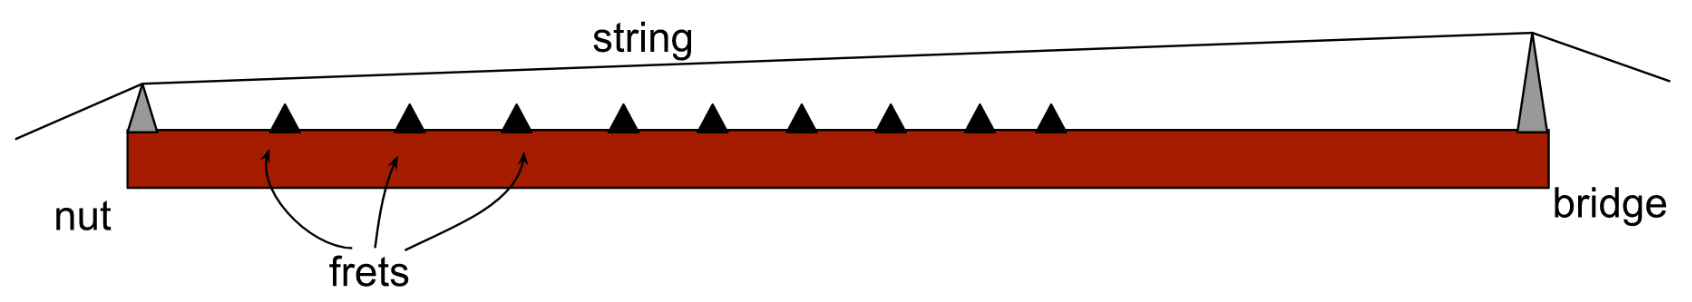
\includegraphics[width=\textwidth]{./ee/fig1.png}
    \caption{A simplified model of the electric guitar I will use. The pickup is not shown.}\label{fig1}
\end{figure} 
\FloatBarrier